\documentclass[../ManualeSviluppatore.tex]{subfiles}

\begin{document}

\begin{appendices}
	\label{sec:FondamentiDiAndroid}
	\section{Fondamenti di Android}
		Nella presente sezione si riportano le principali conoscenze di Android utilizzate nell'applicazione e quindi indispensabili per una maggiore e più completa comprensione del manuale.
	
		%\subsection{Ciclo di vita di un'applicazione}
			
		
		\subsection{Activity}
			Un'Activity è una classe offerta dall'Android SDK che ha lo scopo di gestire una schermata della propria applicazione. Ogni view quindi deve essere supportata da una classe che estende \Activity.
		
			\subsubsection{Ciclo di vita}
				Il potenziale di un'Activity risiede nella curata gestione del proprio ciclo di vita e quindi dell'interfaccia grafica associata. Infatti nei dispositivi mobile le applicazioni hanno un diverso ciclo di vita rispetto alle normali applicazioni nei comuni personal computer.
				
				Un'applicazione mobile necessita di essere in diversi stati a seconda dell'interazione dell'utente, garantire una user experience sempre ottimale e sfruttare al meglio le risorse hardware limitate.
				
				I diversi stati di una sottoclasse \Activity\ sono i seguenti:
				\begin{itemize}
					\item \lstinline|onCreate()| metodo invocato alla creazione dell'Activity;
					\item \lstinline|onStart()| metodo invocato per ripartire l'Activity precedentemente abbandonata dall'utente e lasciata
					\item \lstinline|onResume()| metodo invocato quando l'activity ha ripreso ad essere in primo piano;
					\item \lstinline|onPause()| metodo invocato subito dopo che l'Activity perdi il posto in primo piano, per esempio per un pop-up;
					 in background dal sistema operativo;
					\item \lstinline|onStop()| metodo invocato dopo che l'activity lascia il posto ad un'altra;
					\item \lstinline|onDestroy()| metodo invocato nel caso in cui il sistema operativo necessiti di risorse e l'activity non è utilizzata dall'utente.
				\end{itemize}
				
				\begin{figure} [p]
					\centering
					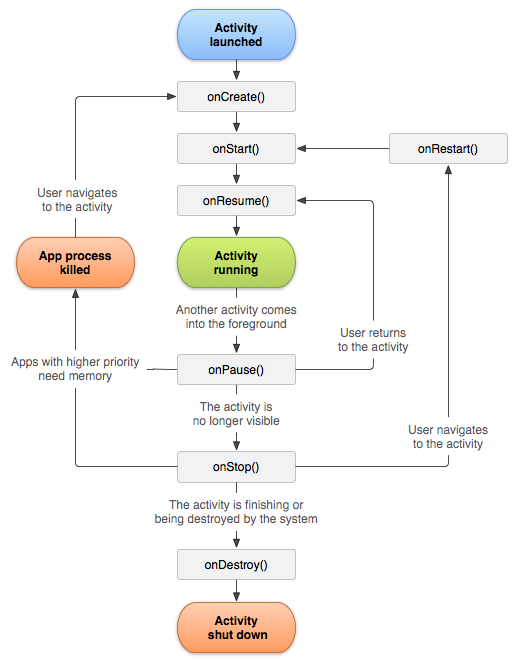
\includegraphics[width=\textwidth]{img/ActivityCiclo}
					\caption{Ciclo di vita Activity}
					\label{fig:ActivityCiclo}
				\end{figure}
			
		\subsection{Service}
			Un Service è una classe offerta dall'Android SDK per poter gestire processi in background in una applicazione con non necessitano di un'interfaccia (come nel caso delle Activity).
		
		Esistono due tipologie di \Service:
			\begin{description}
				\item [unBind Service:] è un Service che comunica con le altre componenti dell'applicazione solo attraverso messaggi \Intent e \BroadcastReceiver;
				\item [Bind Service:] è un Service che rende disponibile la possibilità di ottenere un riferimento su di esso e quindi di invocare metodi implementati da esso stesso. Questa comunicazione avviene attraverso l'uso dell'\IBinder.
			\end{description}
		
			\subsubsection{Ciclo di vita}
				Come l'Activity anche il \Service\ mette a disposizione tutti i metodi per gestire il proprio ciclo di vita in modo da istruire l'applicazione a rispondere alle richieste del sistema operativo, per esempio la richiesta di fermare un Service per liberare risorse.
				I metodi offerti oltre a quelli prima esposti nella sezione Activity sono:
				\begin{itemize}
					\item \lstinline|onStartCommand()| è il metodo invocato quando un'altra componente avvia il Service con la chiamata \lstinline|startService(intent)|, spesso un'Activity.
					\item \lstinline|onBind()| è il metodo messo a disposizione dal Bind Service per poter restituire un riferimento al Service stesso.
				\end{itemize}
				
				\begin{figure} [p]
					\centering
					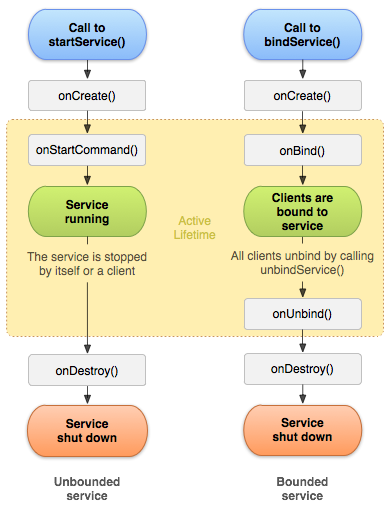
\includegraphics[width=\textwidth]{img/ServiceCiclo}
					\caption{Ciclo di vita unBind Service e Bind Service}
					\label{fig:ServiceCiclo}
				\end{figure}
				
\end{appendices}
\end{document}
